\documentclass[11pt]{article}  
\usepackage[margin=1in]{geometry}
\parindent=0in
\parskip=8pt
\usepackage{fancyhdr,amssymb,amsmath, graphicx, listings,float,subfig,enumerate,epstopdf,color,multirow,setspace,bm,textcomp}
\usepackage[usenames,dvipsnames]{xcolor}
\usepackage{hyperref}
\usepackage{graphicx}
\graphicspath{{./Images}}

\pagestyle{fancy}


\begin{document} 

\lhead{Assignment \# 2}
\chead{Robert Denim Horton}
\rhead{\today}

\begin{center}\begin{Large}
CS 4720/5720 Design and Analysis of Algorithms

Homework \#2

Student: (Robert Denim Horton)
\end{Large}
\end{center}


\section*{Answers to homework problems:}

\begin{enumerate}
% Question 2
\item Consider the graph in Figure 3.21, in which each edge - except the edge connecting $b$ and $c$ - is labeled as a strong tie (S) or a weak tie (W).\\
\begin{center}
	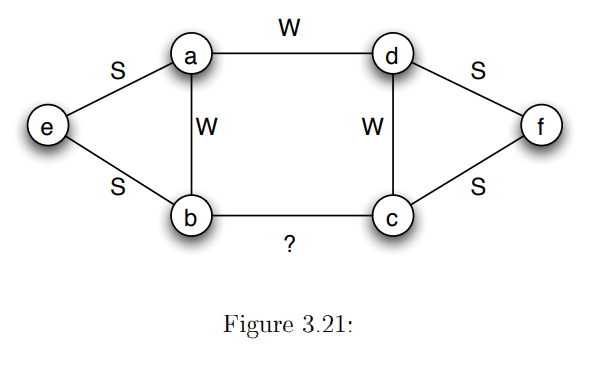
\includegraphics[scale=0.6]{Figure_3_21}
\end{center}
According to the theory of strong and weak ties, with the strong triadic closure assumption, how would you expect the edge connecting b and c to be labeled? Give a brief (1-3 sentence) explanation for your answer.
% Question 3
\item  In the social network depicted in Figure 3.22, with each edge labeled as either a strong or weak tie, which nodes satisfy the Strong Triadic Closure Property from Chapter 3, and which do not? Provide an explanation for your answer
\begin{center}
	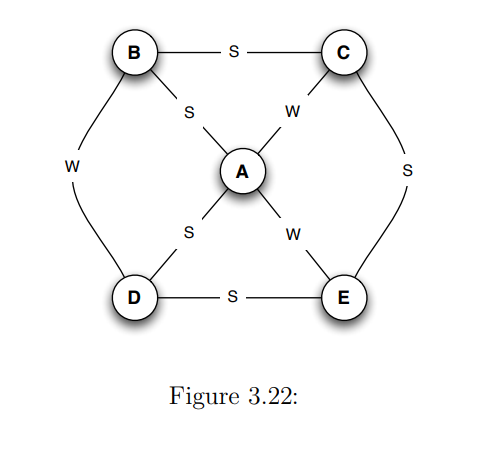
\includegraphics[scale=0.6]{Figure_3_22}
\end{center}
% Question 4
\item In the social network depicted in Figure 3.23 with each edge labeled as either a strong or weak tie, which two nodes violate the Strong Triadic Closure Property? Provide an explanation for your answer
\begin{center}
	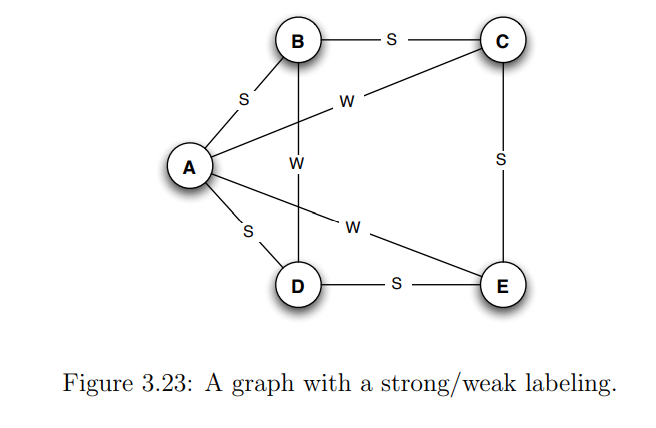
\includegraphics[scale=0.6]{Figure_3_23}
\end{center}
% Question 5
\item  In the social network depicted in Figure 3.24, with each edge labeled as either a strong or weak tie, which nodes satisfy the Strong Triadic Closure Property from Chapter 3, and which do not? Provide an explanation for your answer.
\begin{center}
	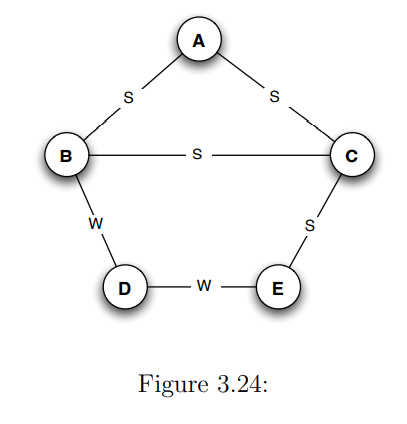
\includegraphics[scale=0.6]{Figure_3_24}
\end{center}
\end{enumerate}
\end{document}
